%%%%%%%%%%%%%%%%%%%%%%%%%%%%%%%%%%%%%%%%%%%%%%%%%%%%%%%%%%%%%%%%%%%%%%%%%%%%%%%%%%%%%%%%%%%%%%%%%%%%%%%%%%%%%%%%%%%%%%%%%%%%%%%%%%%%%%%%%%%%%%%%%%%%%%%%%%%%%%%%%%%
% Written By Michael Brodskiy
% Class: Embedded Design: Enabling Robotics
% Professor: S. Shazli
%%%%%%%%%%%%%%%%%%%%%%%%%%%%%%%%%%%%%%%%%%%%%%%%%%%%%%%%%%%%%%%%%%%%%%%%%%%%%%%%%%%%%%%%%%%%%%%%%%%%%%%%%%%%%%%%%%%%%%%%%%%%%%%%%%%%%%%%%%%%%%%%%%%%%%%%%%%%%%%%%%%

\documentclass[12pt]{article} 
\usepackage{alphalph}
\usepackage[utf8]{inputenc}
\usepackage[russian,english]{babel}
\usepackage{titling}
\usepackage{amsmath}
\usepackage{graphicx}
\usepackage{enumitem}
\usepackage{amssymb}
\usepackage[super]{nth}
\usepackage{everysel}
\usepackage{ragged2e}
\usepackage{geometry}
\usepackage{multicol}
\usepackage{fancyhdr}
\usepackage{cancel}
\usepackage{siunitx}
\usepackage{physics}
\usepackage{lastpage}
\usepackage{tikz}
\usepackage{mathdots}
\usepackage{yhmath}
\usepackage{cancel}
\usepackage{color}
\usepackage{array}
\usepackage{multirow}
\usepackage{gensymb}
\usepackage{tabularx}
\usepackage{extarrows}
\usepackage{booktabs}
\usetikzlibrary{fadings}
\usetikzlibrary{patterns}
\usetikzlibrary{shadows.blur}
\usetikzlibrary{shapes}

\geometry{top=1.0in,bottom=1.0in,left=1.0in,right=1.0in}
\newcommand{\subtitle}[1]{%
  \posttitle{%
    \par\end{center}
    \begin{center}\large#1\end{center}
    \vskip0.5em}%

}
\usepackage{hyperref}
\hypersetup{
colorlinks=true,
linkcolor=blue,
filecolor=magenta,      
urlcolor=blue,
citecolor=blue,
}

\pagestyle{fancy}

\lfoot[\vspace{-15pt} \hline]{\vspace{-15pt} \hline}
\rfoot[\vspace{-15pt} \hline]{\vspace{-15pt} \hline}
\cfoot[\thepage]{\thepage}
\chead[\textsc{Embedded Systems}]{\textsc{Embedded Systems}}
\lhead[\textsc{EECE2160, CRN: 32014}]{\textsc{EECE2160, CRN: 32014}}
\rhead[\textsc{Page \thepage \hspace{1pt} of \pageref{LastPage}}]{\textsc{Page \thepage \hspace{1pt} of \pageref{LastPage}}}



\pagestyle{fancy}

\title{Digital Logic Minimization for Lab 2}
\date{\today}
\author{Michael Brodskiy\\ \small Professor: S. Shazli}

\begin{document}

\maketitle

\thispagestyle{fancy}

\newpage

\begin{itemize}

  \item Don't Care Entry: ``x'' means the entry is not relevant either at input or output

  \item In other words, we are free to assign either 0 or 1 to reduce the Boolean expression

  \item Example:

    \begin{center}
      \begin{tabular}[h!]{l | c c c | r}
        ID & a & b & c & f(a,b,c)\\
        \hline
        0 & 0 & 0 & 0 & 0\\
        1 & 0 & 0 & 1 & 0\\
        2 & 0 & 1 & 0 & 1\\
        3 & 0 & 1 & 1 & 0\\
        4 & 1 & 0 & 0 & 1\\
        5 & 1 & 0 & 1 & 1\\
        6 & 1 & 1 & 0 & $\boxed{x}$\\
        7 & 1 & 1 & 1 & 1\\
      \end{tabular}
    \end{center}

  \item Extending this to our second lab, we get:

\begin{center}
  \begin{tabular}[H]{| c || c | c | c | c || c | c | c | c | c | c | c |}
    \hline
    \# & In3 & In2 & In1 & In0 & a & b & c & d & e & f & g \\
    \hline
    0 & 0 & 0 & 0 & 0 & 0 & 0 & 0 & 0 & 0 & 0 & 1 \\
    \hline 
    1 & 0 & 0 & 0 & 1 & 1 & 0 & 0 & 1 & 1 & 1 & 1 \\
    \hline
    2 & 0 & 0 & 1 & 0 & 0 & 0 & 1 & 0 & 0 & 1 & 0 \\
    \hline
    3 & 0 & 0 & 1 & 1 & 0 & 0 & 0 & 0 & 1 & 1 & 0\\
    \hline
    4 & 0 & 1 & 0 & 0 & 1 & 0 & 0 & 1 & 1 & 0 & 0\\
    \hline
    5 & 0 & 1 & 0 & 1 & 0 & 1 & 0 & 0 & 1 & 0 & 0\\
    \hline
    6 & 0 & 1 & 1 & 0 & 0 & 1 & 0 & 0 & 0 & 0 & 0\\
    \hline
    7 & 0 & 1 & 1 & 1 & 0 & 0 & 0 & 1 & 1 & 1 & 1\\
    \hline
    8 & 1 & 0 & 0 & 0 & 0 & 0 & 0 & 0 & 0 & 0 & 0\\
    \hline
    9 & 1 & 0 & 0 & 1 & 0 & 0 & 0 & 0 & 1 & 0 & 0\\
    \hline
  \end{tabular}
\end{center}

    \item Here, a 1 represents off and a 0 represents on

    \item A seven-segment display is an electronic component that displays a 1-digit number from 0-9 and a letter A to F

    \item In this lab, we will design a circuit to display digits 0 to 9 only using digital logic components

    \item The circuit we will design is called a Binary Coded Decimal (BCD) decoder 
      
    \item This circuit takes in a 4-bit input representing the binary equivalent of a digit 0 to 9 and lights up the desired segments to display the corresponding digit 
      
    \item The segment can be turned on or off by applying a low logic level or high logic level from the FPGA, respectively

    \item This is according to a 7-segment BCD system, as seen in Figure \ref{fig:1}

      \begin{figure}[h!]
        \centering
        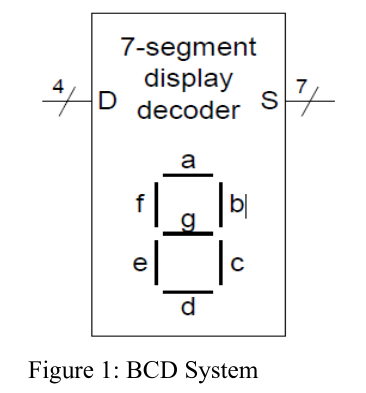
\includegraphics[width=.3\textwidth]{Figures/BCD.png}
        \label{fig:1}
      \end{figure}

      \newpage

    \item Numbers in a seven segment display are constructed as shown in Figure \ref{fig:2}

      \begin{figure}[h!]
        \centering
        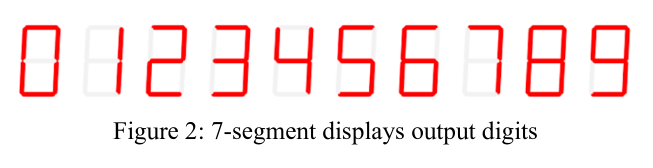
\includegraphics[width=.85\textwidth]{Figures/7SD.png}
        \label{fig:2}
      \end{figure}

    \item Constructing a Karnaugh map for a in the table above, we get:

    \begin{center}
      \begin{tabular}[h!]{|c | c | c | c | c |}
        \hline
        In3In2 \textbackslash  In1In0 & 00 & 01 & 11 & 10\\
        \hline
        00 & 0 & 1 & 0 & 0\\
        \hline
        01 & 1 & 0 & 0 & 0\\
        \hline
        11 & x & x & x & x\\
        \hline
        10 & 0 & 0 & x & x\\
        \hline
      \end{tabular}
    \end{center}

  \item Using the table, we can simplify the equation to: In2In1'In0' + In3'In2'In1'In0

  \item Thus, the boolean equation produced is simplified and correct

  \item This is written in terms of a sum of products

  \item The equation has been minimized through graphical means

  \item Now, the same steps need to be applied to the BCD-based table

  \item This will have to be done for each variable that is left

    \newpage

  \item For b:

    \begin{center}
      \begin{tabular}[h!]{|c | c | c | c | c |}
        \hline
        In3In2 \textbackslash  In1In0 & 00 & 01 & 11 & 10\\
        \hline
        00 & 0 & 0 & 0 & 0\\
        \hline
        01 & 0 & 1 & 0 & 1\\
        \hline
        11 & x & x & x & x\\
        \hline
        10 & 0 & 0 & x & x\\
        \hline
      \end{tabular}
    \end{center}

  \item This results in: In2In1'In0 + In2In1In0'

  \item For c:

    \begin{center}
      \begin{tabular}[h!]{|c | c | c | c | c |}
        \hline
        In3In2 \textbackslash  In1In0 & 00 & 01 & 11 & 10\\
        \hline
        00 & 0 & 0 & 0 & 1\\
        \hline
        01 & 0 & 0 & 0 & 0\\
        \hline
        11 & x & x & x & x\\
        \hline
        10 & 0 & 0 & x & x\\
        \hline
      \end{tabular}
    \end{center}

  \item This results in: In3'In2'In1In0'

  \item For d:

    \begin{center}
      \begin{tabular}[h!]{|c | c | c | c | c |}
        \hline
        In3In2 \textbackslash  In1In0 & 00 & 01 & 11 & 10\\
        \hline
        00 & 0 & 1 & 0 & 0\\
        \hline
        01 & 1 & 0 & 1 & 0\\
        \hline
        11 & x & x & x & x\\
        \hline
        10 & 0 & 0 & x & x\\
        \hline
      \end{tabular}
    \end{center}

  \item This results in: In2In1'In0' + In3'In2'In1'In0 + In2In1In0

  \item For e:

    \begin{center}
      \begin{tabular}[h!]{|c | c | c | c | c |}
        \hline
        In3In2 \textbackslash  In1In0 & 00 & 01 & 11 & 10\\
        \hline
        00 & 0 & 1 & 1 & 0\\
        \hline
        01 & 1 & 1 & 1 & 0\\
        \hline
        11 & x & x & x & x\\
        \hline
        10 & 0 & 1 & x & x\\
        \hline
      \end{tabular}
    \end{center}

  \item This results in: In2In1'In0' + In0

  \item For f:

    \begin{center}
      \begin{tabular}[h!]{|c | c | c | c | c |}
        \hline
        In3In2 \textbackslash  In1In0 & 00 & 01 & 11 & 10\\
        \hline
        00 & 0 & 1 & 1 & 1\\
        \hline
        01 & 0 & 0 & 1 & 0\\
        \hline
        11 & x & x & x & x\\
        \hline
        10 & 0 & 0 & x & x\\
        \hline
      \end{tabular}
    \end{center}

  \item This results in: In3'In2'In0 + In3'In2'In1 + In3'In1In0

  \item For g:

    \begin{center}
      \begin{tabular}[h!]{|c | c | c | c | c |}
        \hline
        In3In2 \textbackslash  In1In0 & 00 & 01 & 11 & 10\\
        \hline
        00 & 1 & 1 & 0 & 0\\
        \hline
        01 & 0 & 0 & 1 & 0\\
        \hline
        11 & x & x & x & x\\
        \hline
        10 & 0 & 0 & x & x\\
        \hline
      \end{tabular}
    \end{center}

  \item This results in: In3'In2'In1' + In2In1In0

\end{itemize}

\end{document}

